\chapter{ Utility Battery Energy Storage - Energy Arbitrage Only}
\label{sec:energy_arbitrage}
In the most elementary form, energy arbitrage entails charging when the wholesale spot price is low, and discharging when the wholesale price is high. Whilst conceptually simple, the purchase price of a battery is high, and there are physical limitations on charge/discharge and the frequency of high spot prices is relatively infrequent.
\section{ Algorithm and Software Selection }
\parencite{McConnell} used COIN-OR Linear Program solver to find the optimal dispatch for a battery performing energy arbitrage. Linear programming is one of the most common optimisation techniques. Leonard Kantrovich was awarded the 1975 Nobel Price in Economics for the optimal allocation of resources using linear programming \parencite{PythonPulp}. Examples of problems that can be solved by linear programming include:
\begin{itemize}
    \item Scheduling – Rota or Factory scheduling to meet production/workload demands at lowest cost
    \item Resourcing Problems – How best to allocate resources to maximise profits
    \item Sudoku
\end{itemize}
PuLP is a suitable tool to perform LP in this thesis for the following reasons: 
\begin{itemize}
    \item Library for Python which is a highly supported coding language with an emphasis on rapid development, clarity of code and a simple object model. 
    \item PuLP works entirely within the syntax of Python and represents optimisation problems and decision variables in  a way that is very similar to the original mathematical expression. 
    \item PuLP is available under a permissive open-source license that encourages and facilitates the use of PuLP inside other projects that need linear optimisation capabilities.
\end{itemize}
\newpage
\section{ Methodology }
The following algorithm represents the methodology for optimising energy arbitrate in a deterministic model with perfect foresight of energy prices over the optimisation window.
\begin{align*}
  \max \sum_{i=0}^T \left(x^{(i)}_c + x^{(i)}_d \right) p^{(i)} \times \left( \frac{l}{60} \right)
\end{align*}
Subject to the constraints:
\begin{alignat} {2}
    -P_{max} &\leq x^{(i)}_c \leq 0  &&\forall i \in [0,T]\\
    0 &\leq x^{(i)}_d \leq P_{max}  &&\forall i \in [0,T]\\
    0 &\leq E^{(i)} \leq E_{max} &&\forall i \in [0,T] \\
    E^{(0)} &= E_{\text{init}} - \left(x^{(0)}_c \eta_c + x^{(0)}_d \frac{1}{\eta_d} \right) \frac{l}{60} && \\
    E^{(i)} &= E^{(i-1)} - \left(x^{(i)}_c \eta_c + x^{(i)}_d \frac{1}{\eta_d} \right) \frac{l}{60} \hspace{1cm} &&\forall i \in [1,T] 
\end{alignat}
Where,
{\renewcommand{\arraystretch}{2}}
\begin{center}
    \begin{tabular}{p{0.8cm} p{5.5cm} p{0.8cm} p{5.5cm}}
    \textbf{Constants} & & \textbf{Variables} & \\
    $P_{max}$ & Power Capacity of BESS (MW) & $x^{(i)}_c$ & Charge power at time $i$ (MW)   \\ 
    $E_{max}$ & Storage Capacity of BESS (MWh) & $x^{(i)}_c$&  Discharge power at time $i$ (MW)  \\
    $E_{\text{init}}$ & Initial Storage Level of BESS (MWh)& $E^{(i)}$ &Storage level at time $i$ (MWh)\\
    $l$ & length of time interval in minutes & & \\
    $\eta_c$ & Charge efficiency (\%) & &\\
    $\eta_d$ & Discharge efficiency (\%) & &\\
    $p^{(i)}$ &  Energy price at time $i$ (\$/MWh) & &\\
    $T$ &  Total number of time intervals & &\\
    \end{tabular}
\end{center}
To implement this algorithm, the following methodology was undertaken;
\begin{enumerate}
    \item Configure a Python 3.7 environment.
    \item Import price data via NEMOSIS:  \url{https://github.com/UNSW-CEEM/NEMOSIS}. NEMOSIS is a simple tool for creating datasets using publicly available information about the Australian National Electricity Market (NEM).
    \item Create a battery object.
    \item PuLP python optimisation problem formulation;
    \begin{enumerate}
        \item Identify the Decision Variables
        \item Formulate the Objective Function using the decision variables
        \item Formulate the Constraints
    \end{enumerate}
\end{enumerate}
It is crucial to note that the energy arbitrage only model assumes the battery is a price-taker, and has perfect foresight of price.
\section{ Analysis }
\subsection{ Method Validation }
As shown in Figure \ref{fig:simple_output}, the dispatch logic charging during low prices, and discharging during high prices is effective. Note in Figure \ref{fig:simple_output} a single trip efficiency of 90\% or round trip efficiency of 81\% is implemented. This is a conservative measure, with Tesla stating their Power Pack round trip efficiency is 88\% \url{https://www.tesla.com/en_AU/powerpack}. 
\begin{figure}[H]
    \centering
    \makebox[\textwidth][c]{    \includegraphics[width=1.1\textwidth]{"Pictures/Chapter3/battery_plot".pdf}}
    \caption{BESS Output - 2018-01-01}
    \label{fig:simple_output}
\end{figure}
In order to validate the model, \parencite{Wang} provides energy arbitrage revenues for a 1MW ESS with capacity between 1-8MWh, using NEM price data for years 2010-2013 with perfect foresight. The model assumes 90\% single trip efficiency. The findings are summarised in Figure \ref{fig:wang_ea}. 
\begin{figure}[H]
    \centering
    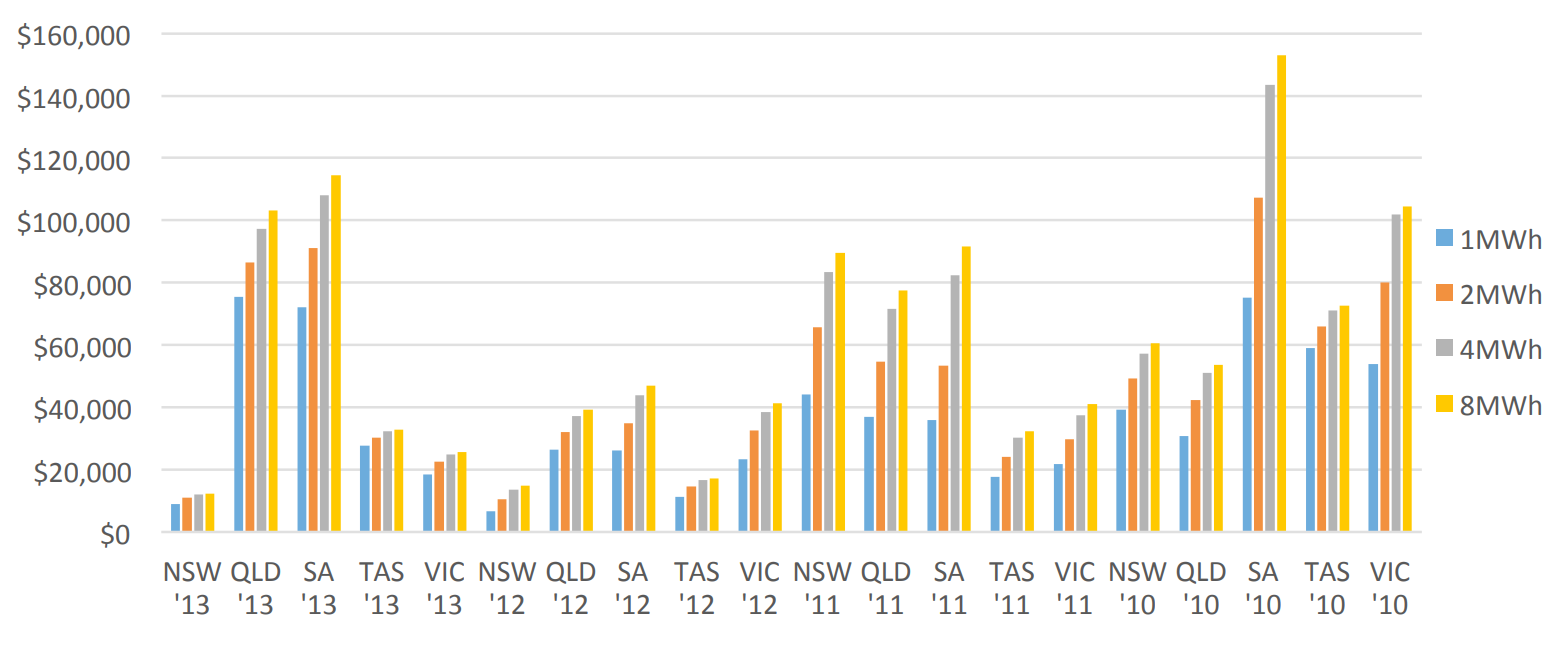
\includegraphics{Pictures/Chapter3/wang_ea.PNG}
    \caption{Energy Arbitrage - Geographic and Temporal Comparison (Wang 2016)}
    \label{fig:wang_ea}
\end{figure}
Below, Figure \ref{fig:wang_ea_comparion} is the implementation of the python (pyBess) model replicating Wang's results. 
\begin{figure}[H]
    \centering
    \makebox[\textwidth][c]{    \includegraphics[width=1\textwidth]{"Pictures/Chapter3/ae_wang_comparison".pdf}}
    \caption{Energy arbitrage annual revenue for a 1 MW / 1 MWh BESS by region 2010 - 2013}
    \label{fig:wang_ea_comparion}
\end{figure}
\begin{wrapfigure}{r}{0.6\textwidth}
    \begin{center}
        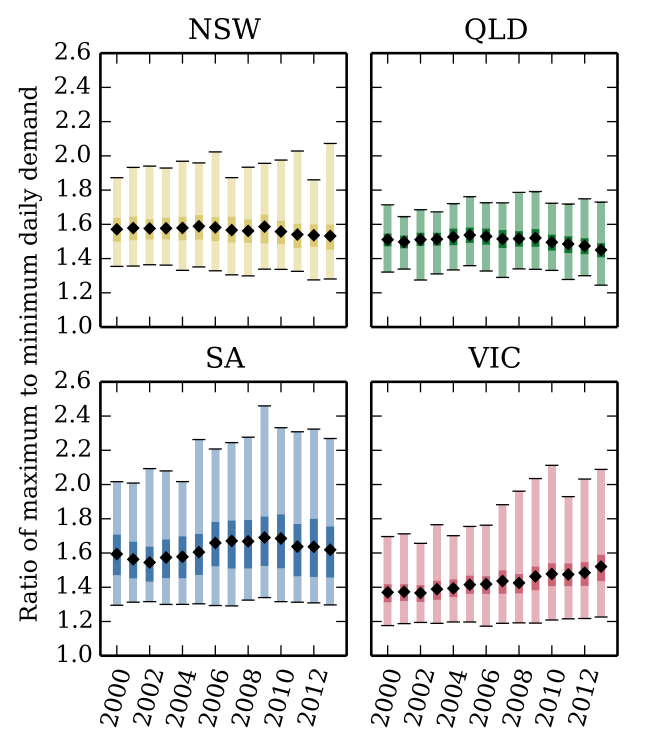
\includegraphics[width=0.4\textwidth]{Pictures/Chapter3/energy_vol.png}
    \end{center}
    
    \caption{National Electricity Market Demand Volatility \parencite{McConnell}}
    \label{fig:demand_volatility}
\end{wrapfigure}
Given Figures \ref{fig:wang_ea} and \ref{fig:wang_ea_comparion} exhibit identical characteristics, this validates the energy only model. This preliminary example also highlights a number of key findings;
\begin{enumerate}
    \item NSW is on average the worst performing state for energy arbitrage.
    \item SA is consistently a high performer relative to other states.
    \item Large discrepancies can occur year-to-year.
    \item Additional storage which increases the cost of a battery proportionally offers diminishing returns for all example. This indicates that short price spikes generally drive revenue, rather than sustained high prices periods. 
\end{enumerate}
Figure \ref{fig:demand_volatility} provided by \textcite{McConnell} highlights the daily variation in demand for each NEM jurisdiction (excl. TAS). Demand volatility which inherently drives price volatility, generally reflects economic and climatic factors. As shown in Figure \ref{fig:demand_volatility}, South Australia has the highest ratio of maximum to minimum daily demand.  
\subsection{ Dependency on Price Dynamics }
Figure \ref{fig:revenue_duration} displays a revenue duration curve of a 1MW/1MWh BESS with 90\% round-trip efficiency from FY 2010 - 2017. The logarithmic scale clearly indicates that less than 10\% of the time, a very significant proportion of revenue is raised from infrequent, high price events. Figure \ref{fig:revenue_duration} also demonstrates an increase in overall BESS revenue - beyond 2013 (not reflected in Figure \ref{fig:wang_ea_comparion}). 
\begin{figure}[H]
    \centering
    \makebox[\textwidth][c]{    \includegraphics[width=1\textwidth]{"Pictures/Chapter3/Revenue Duration Curve for FY10 - FY17".pdf}}
    \caption{Revenue Duration Curve for FY10 - FY17}
    \label{fig:revenue_duration}
\end{figure}
\begin{wrapfigure}{r}{0.6\textwidth}
    \begin{center}
        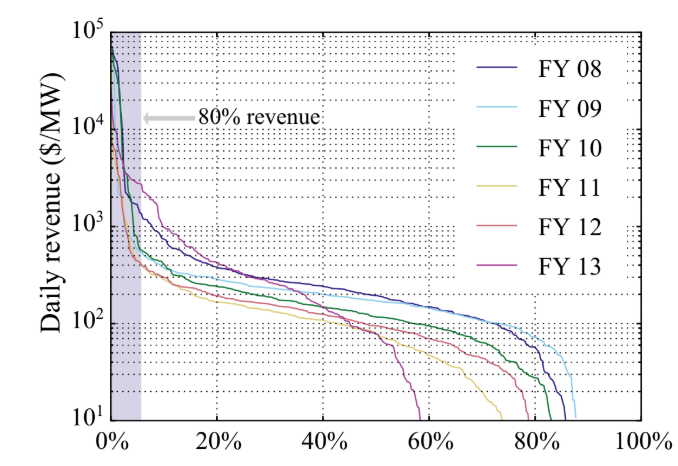
\includegraphics[width=0.6\textwidth]{Pictures/Chapter3/mcconnell_revenue_duration.png}
    \end{center}
    \caption{BESS Revenue Duration Curve (McConnell 2014)}
    \label{fig:mcconnell_rev_duration}
\end{wrapfigure}
 Again, the work of McConnell reinforces this notion in Figure  \ref{fig:mcconnell_rev_duration}. Overall, this phenomenon is expected due to the high Market Clearing Price (MCP) of the NEM at \$14,500.  A high MCP is an essential ingredient to electricity market design. In case of scarcity situations and extreme market fundamentals – such as a heat wave in South Australia, prices may sore to \$14,500/MWh for a number of intervals. This might sound extreme, but have been observed from time to time in the past few years. Such economically justified scarcity prices have a negligible impact on the average price of
electricity for end consumers – however, they are vital for the profitability of flexible power plants \parencite{scarcity_pricing}. 
\subsection{ Seasonal Impact }
Figure \ref{fig:mcconnell_heatmap} illustrates the average optimal operating regime for different hours of the day and different days of the year in South Australia. As expected, the dispatch follows the seasonal price and demand patterns characterised by a bi-modal peak in winter and an afternoon peak in summer.
\begin{figure}[H]
    \centering
    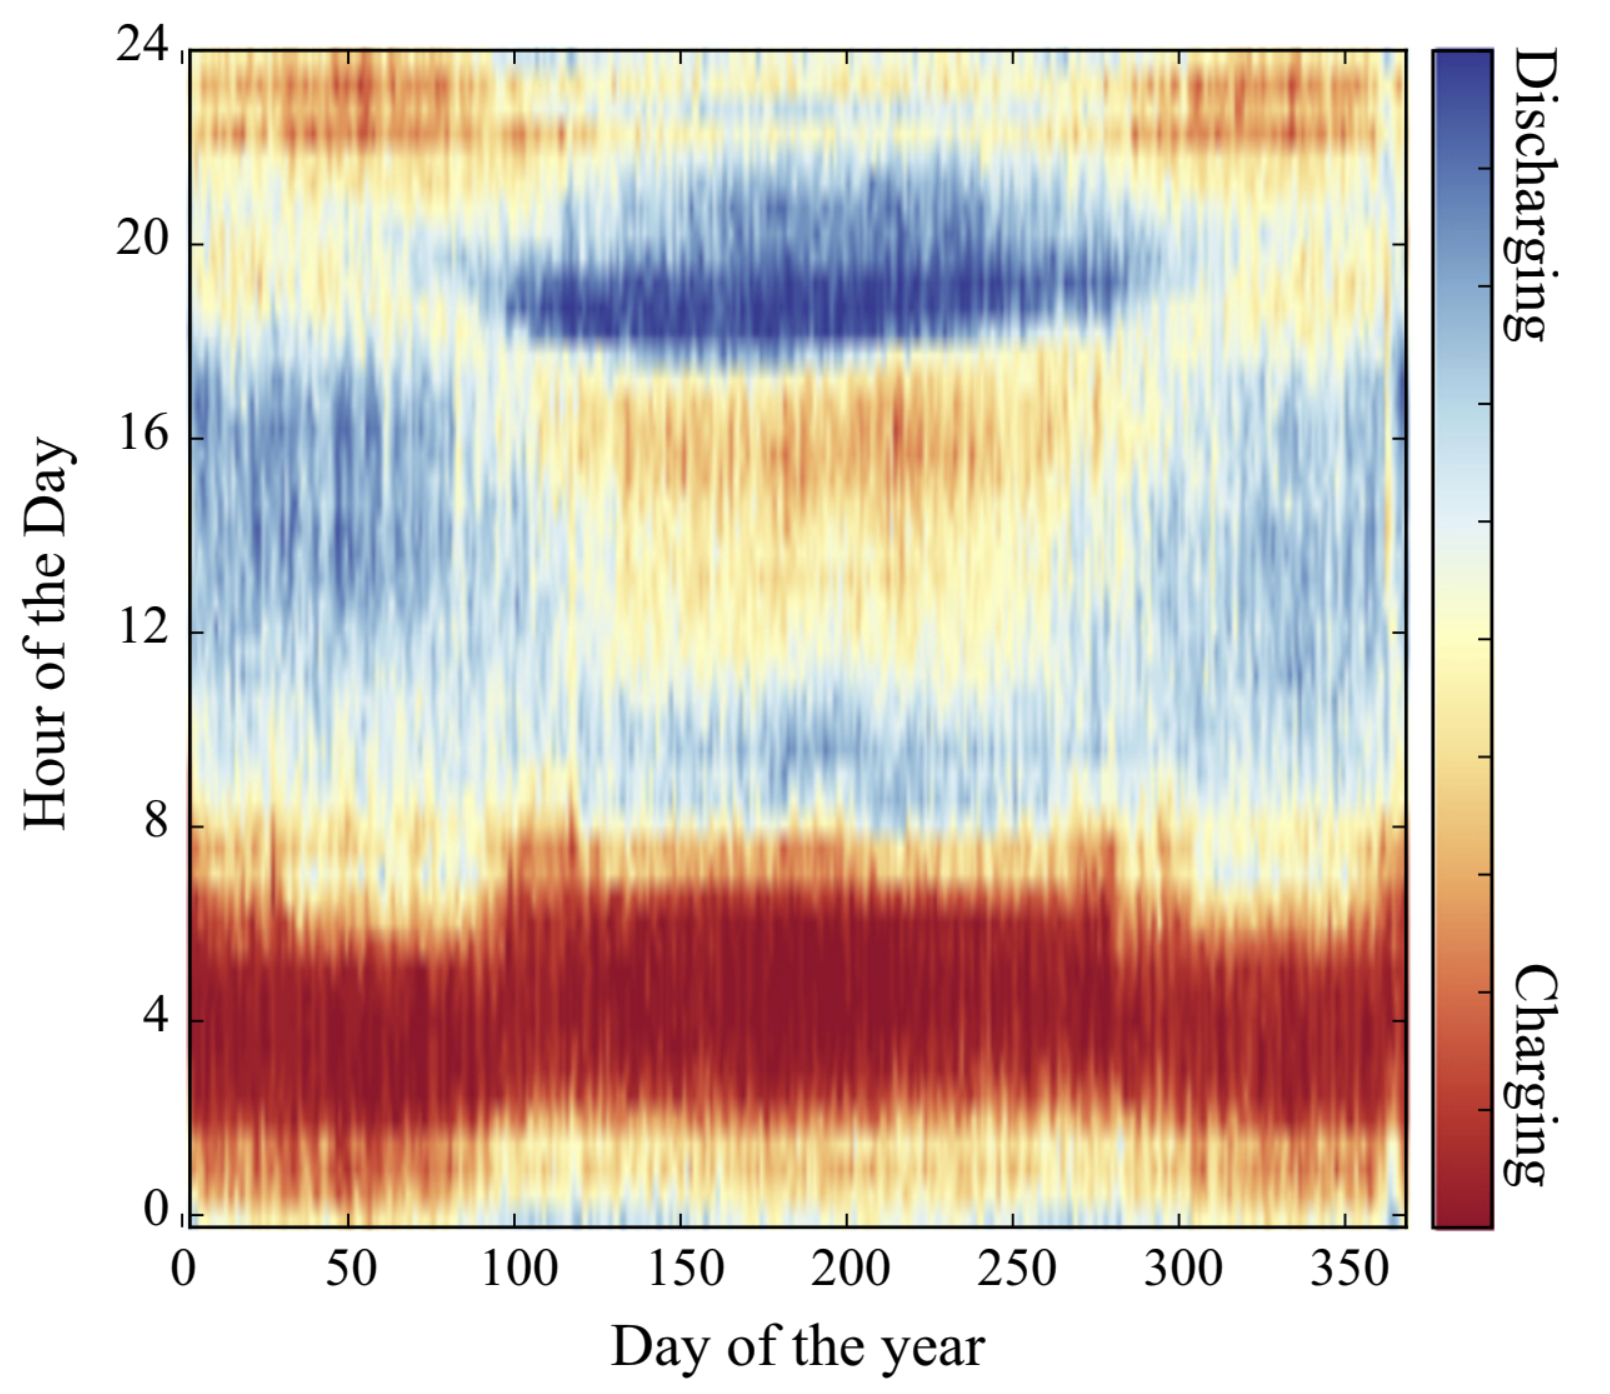
\includegraphics[width=0.6\textwidth]{Pictures/Chapter3/mcconnel_heatmap.png}
    \caption{Optimal BESS operation characteristics, for winter and summer months of the year. (McConnell, 2015)}
    \label{fig:mcconnell_heatmap}
\end{figure}
Figure \ref{fig:heatmap} extends the analysis of McConnell, demonstrating the impact that storage capacity has on operating characteristics. The contrast in both sides of the subplot is that 1 Hour storage often has idle times (cream colour) whilst 8 Hours of storage is constantly either charging or discharging.
\begin{figure}[H]
    \centering
    \makebox[\textwidth][c]{    \includegraphics[width=1\textwidth]{"Pictures/Chapter3/South Australia - 2017".pdf}}
    \caption{Optimal BESS operation characteristics, for winter and summer months of the year, varying storage capacity.}
    \label{fig:heatmap}
\end{figure}
\subsection{ Impact of Throughput Constraints }
Below Figure \ref{fig:throughput_limit} shows the impact of applying a 365 cycles per annum throughput limit on a battery energy storage system. As shown, for both region and storage capacity - throughput limitations typically don't hinder arbitrage revenues significantly. 
\begin{figure}[H]
    \centering
    \makebox[\textwidth][c]{    \includegraphics[width=1\textwidth]{"Pictures/Chapter3/Impact of Throughput on Annual Revenue_ 1 MW Battery".pdf}}
    \caption{Impact of Throughput on Annual Revenue: 1 MW Battery}
    \label{fig:throughput_limit}
\end{figure}
\subsection{ Recent Trends and Driving Factors for Energy Arbitrage Revenue }
\label{sec:trends}
Figure \ref{fig:wang_plot_full} extends Figure \ref{fig:wang_ea_comparion} and shows the energy arbitrage revenue with perfect foresight, for a 1MW BESS including the calendar years (15,16,17,18). 
\begin{figure}[H]
    \centering
    \makebox[\textwidth][c]{    \includegraphics[width=1\textwidth]{"Pictures/Chapter3/Energy Arbitrage - Geographic and Temporal Comparison".pdf}}
    \caption{Energy arbitrage annual revenue for a 1 MW / 1 MWh BESS by region 2010 - 2018}
    \label{fig:wang_plot_full}
\end{figure}
\begin{wrapfigure}{r}{0.6\textwidth}
    \begin{center}
        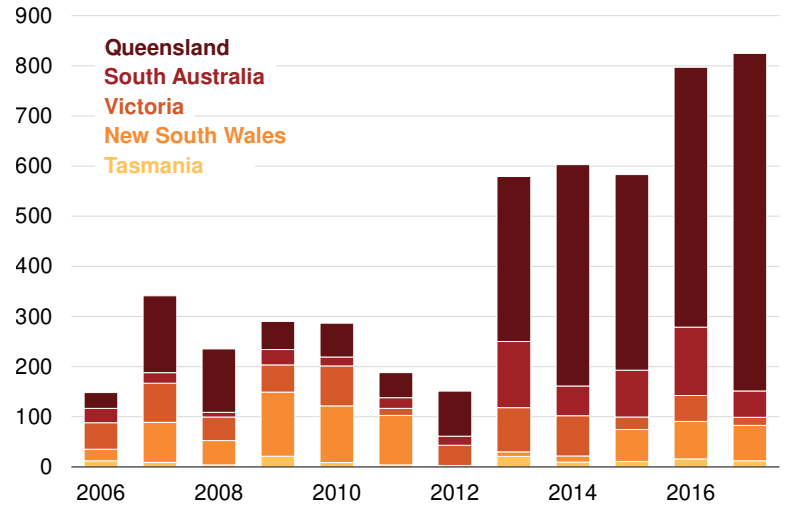
\includegraphics[width=0.6\textwidth]{Pictures/Chapter3/generator_gaming.png}
    \end{center}
    \caption{Increase in total value traded in the NEM from bidding games, \$ millions (Grattan Institute, 2018)}
    \label{fig:generator_gaming}
\end{wrapfigure}
Figure \ref{fig:wang_plot_full} highlights a number of key findings. Firstly. Since 2014, the arbitrage value of battery energy storage has clearly increased. 
\newline
Secondly, 2016 witnessed the highest revenues,  especially in South Australia.  \parencite{2016_prices} described the driving force behind the high volatility in 2016 attributable to the removal of the Northern Power Station. \textcite{2016_prices} also highlights a combination of high winter demand, low wind generation, planned upgrades to the Heywood interconnector, in combination with low levels of gas fired generation that coincided with high gas prices all contributed to high volatility.
\newline
Thirdly, Queensland in 2017 exhibited the highest revenue across the states. \parencite{grattan} attributes such volatility in 2017 to Queensland’s government-owned generation companies, Stanwell Corporation and CS Energy, (who provided 71 per cent of all electricity in Queensland in 2016–17), and reported record profitability; 30.4 and 58.9 per cent ROE, respectively. As shown in Figure \ref{fig:generator_gaming}, the value of bidding games have drastically increased in Queensland over the past decade. Gaming in the NEM can cause extreme price fluctuations, as shown in Figure \ref{fig:generator_gaming_1}. Figure \ref{fig:generator_gaming_1} highlights seven dispatch intervals that were near the market price cap of \$14,200/MWh, while most dispatch intervals were around \$100/MWh. In June 2017, the Queensland Government announced
the Powering Queensland Plan, which included a directive to Stanwell Corporation to \textit{“undertake strategies to place downward pressure on
wholesale prices"}. This aligns with Figure \ref{fig:wang_plot_full} as QLD 2018 revenues drop below NSW for the first time since 2011.
\begin{figure}
    \centering
    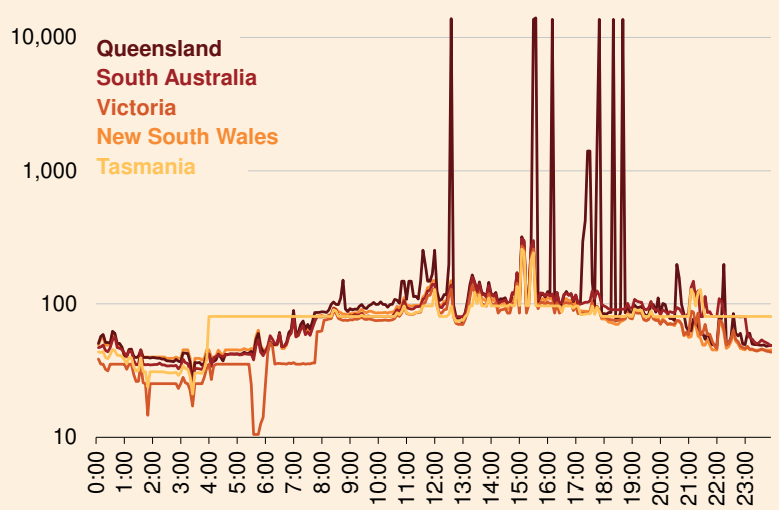
\includegraphics[width=0.6\textwidth]{Pictures/Chapter3/generator_gaming_2.png}
    \caption{5-minute dispatch interval
price by state for 12 January 2017 (Wood, 2018)}
    \label{fig:generator_gaming_1}
\end{figure}
\section{ Performance under a Changing Generation Mix}
\label{generation_mix}
Section \ref{sec:trends} highlights the historic trends and emphasises that South Australia is the best performing state for energy arbitrage in the NEM. South Australia has undergone rapid energy transformation over the past 10 years, with exit of coal generators in 2016 \parencite{sa_coal}, uptake of variable renewable energy resources and an increase of behind-the-meter household photovoltaics (PV). AEMO estimates behind-the-meter PV in South Australia currently accounts for 930MW. Additionally, AEMO cites this rapid uptake in behind-the-meter PV combined with energy efficiency savings, kept annual operational consumption in South Australia flat at 12,203 GWh in 2017-18, despite underlying population growth. 
\newline
\newline
AEMO now forecasts minimum operational demand in South Australia because low operational demand introduces operational challenges for balancing the power system. Since 2012-13, annual minimum demand has decreased as rooftop PV capacity increased. Furthermore, AEMO forecasts negative minimum demand for the region under certain conditions by 2023-24. 
\begin{figure}[H]
    \centering
    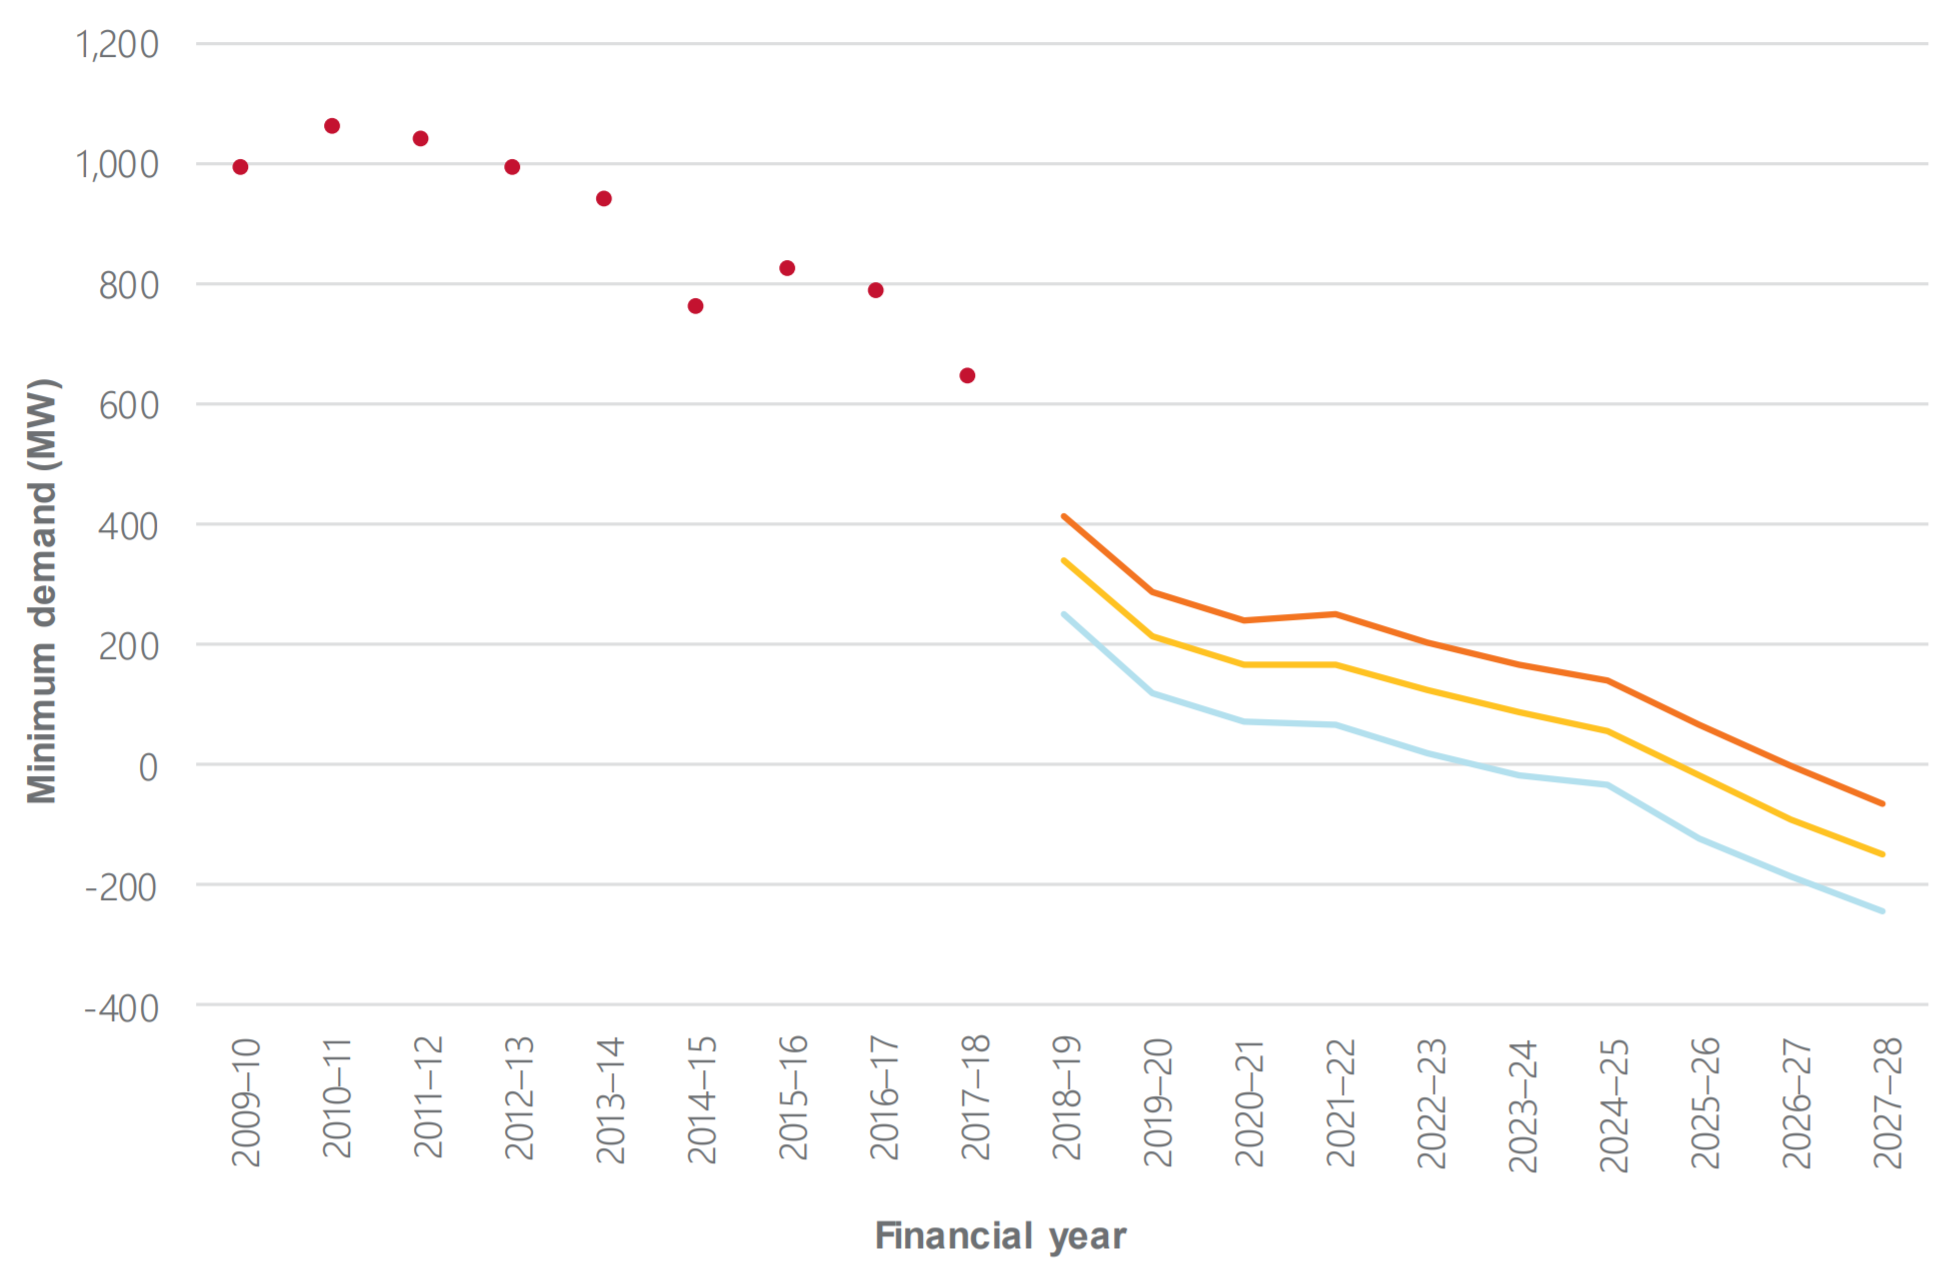
\includegraphics[width=\textwidth]{Pictures/Chapter3/minimum_demand.png}
    \caption{Caption}
    \label{fig:minimum_demand}
\end{figure}
As of July 2017, \textcite{sa_aemo} calculated the nameplate capacity of committed capacity new build utility Solar PV in South Australia as 218 MW; Bungala Two (110 MW) and Tailem Bend Solar Farm (108 MW). However, AEMO also acknowledge an additional 2387.5 MW of Solar PV proposed for the state. Structurally this will have a profound impact of prices during the day exacerbating and already pronounced `duck curve' \footnote{In many energy markets the peak demand occurs after sunset, when solar power is no longer available. In locations where a substantial amount of solar electric capacity has been installed, the amount of power that must be generated from sources other than solar or wind displays a rapid increase around sunset and peaks in the mid-evening hours, producing a graph that resembles the silhouette of a duck}. The following methodology has been undertaken to explore the possible impact that significant additional utility PV will have on South Australia. This method is limited to a narrow scope of additional Solar PV and does not take into account increased investment in Wind, thermal generation technologies or uptake in energy efficiency. Additionally, increased demand in the state or exploration of the proposed SA - NSW interconnector has not been investigated. 
\subsection{ Methodology }
The following steps were undertaken to build 3 scenarios of 30 minute spot prices for South Australia in 2020; a) Business as Usual with no Solar (counterfactual), b) South Australia with an additional 500 MW of Solar c) South Australia with an additional 1000 MW of Solar.
\newline
\textit{Due to commercial confidentiality, this method has been simplified.}
\begin{enumerate}
    \item Random sample (bootstrap) 100 years from 2011-2018 based on month/day-type to construct 100 simulated years of South Australian spot price. 
    \item Re-base the simulated prices such that the average spot price by quarter equals the flat quarterly spot price traded on the ASX spot market for 2020 (As of 04/04/2019).
    \item Generate a single axis PV MW trace by half-hour using NREL's SAM. The location used in the weather file was Port-Augusta.
    \item Generate a regression based on residual demand. The AEMO MMS table was DISPATCHREGIONSOLATION. The regression was based on (totaldemand - semi-scheduled) vs average historic quarterly price. Ultimately this represents a bid stack, and highlights the impact on increasing demand for fossil fuel generators and the impact on price.  Figure \ref{fig:regression} shows the relation for each quarter. As the plot highlights, for each quarter beyond 2000 MW of residual or fossil-fuel demand, South Australia's price quite rapidly tends towards ceiling price, and caps at VoLL around 3000 MW.
    \item Build a counterfactual price trace using the regression model. This involves gathering the 100 simulations of price from the bootstrap set and for each price determine the original price $RRP_1$ (\$/MWh), residual demand $RD_{1}$ (MW), and mean quarterly price for the simulation $QTR_{RRP}$ (\$/MWh).
    The counterfactual price using the residual demand model is given by: 
    \begin{equation}
        RRP_2 = RRP_1 \times \dfrac{MMP_{RD_1}}{MMP_1}
    \end{equation}
    Where $MMP_1$ is the Mean Price Percentage of the original price traces i.e. $100 \times \dfrac{RRP_1}{QTR_{RRP}}$.
    \item To simulate an increase in Solar, we adjust the original residual demand by a the 1MW Solar Trace $S$ multiplied by the MW quantity we require; $RD_{Solar} = RD_1 - N \times S $. We can then find the spot price under additional solar $RRP_S$; 
        \begin{equation}
        RRP_{S} = RRP_1 \times \dfrac{MMP_{RD_S}}{MMP_1}
    \end{equation}
    \item This model was then deployed using 500MW and 1000MW of PV. Figures \ref{fig:bess_w_low_solar} and \ref{fig:bess_w_high_solar} show the impact of the average diurnal price in South Australia using this Solar PV adjustment. As the Figures highlight, additional PV impact peak demand in Q1 and Q4 but doesn't make material difference to the afternoon/evening peak during the winter quarters.  
\end{enumerate}
\begin{figure}[H]
    \centering
    \makebox[\textwidth][c]{    \includegraphics[width=1.15\textwidth]{"Pictures/Chapter6/diurnal_profile_low_solar".pdf}}
    \caption{2020 Re-based SA Price Diurnal Profiles with 500MW MW additional solar PV.}
    \label{fig:bess_w_low_solar}
\end{figure}
\begin{figure}[H]
    \centering
    \makebox[\textwidth][c]{    \includegraphics[width=1.15\textwidth]{"Pictures/Chapter6/diurnal_profile_high_solar".pdf}}
    \caption{2020 Re-based SA Price Diurnal Profiles with 1000 MW additional solar PV.}
    \label{fig:bess_w_high_solar}
\end{figure}
\section{ Analysis }
Figure \ref{fig:bess_w_solar} shows the annual revenue assuming perfect foresight for a 30MW/119MWh BESS under; the 2020 counterfactual scenario, additional 500MW solar scenario and  an additional 1000MW. 30MW/119MWh was chosen as it represents the merchant capactiy of the Hornsdale Power Reserve discussed in Section \ref{hornsdale}.
\begin{figure}[H]
    \centering
    \makebox[\textwidth][c]{    \includegraphics[width=\textwidth]{"Pictures/Chapter6/bess_w_solar".pdf}}
    \caption{30MW/119MW BESS energy arbitrage revenue under 2020 BAU, low and high solar.}
    \label{fig:bess_w_solar}
\end{figure}
From Figure \ref{fig:bess_w_solar} an increase in solar clearly degrades the overall arbitrage by up to 20\% in the 1000 MW scenario. Although additional Solar increases the prevalence of negative pricing during the day, which enables more lucrative and flexible charging regimes, overall demand drive price spikes reduce in magnitude hence reducing overall revenue.
\newline
\newline
This method is only a simple representation of a complex market which is characterised from many physical and economic factors, however this purpose of this section is to illustrate that a evolving generation mix will affect BESS arbitrage revenue, especially in areas where variable intermittent set the marginal clearing price. To explore this in more detail a bottom up approach would offer more insight. In 2018, AEMO released the inaugural Integrated System Plan (ISP) – a comprehensive evaluation of the likely changes that will be occurring over the next 20 years across the National Electricity Market (NEM). Accompanying the ISP is a database which provides a methodology for simulating the NEM over the next 20 years: \url{https://www.aemo.com.au/Electricity/National-Electricity-Market-NEM/Planning-and-forecasting/Integrated-System-Plan/ISP-database}. 